%% LyX 2.1.4 created this file.  For more info, see http://www.lyx.org/.
%% Do not edit unless you really know what you are doing.
\documentclass[english]{article}
\usepackage[T1]{fontenc}
\usepackage[latin9]{inputenc}
\usepackage{amsmath}
\usepackage{graphicx}
\usepackage{esint}

\makeatletter
%%%%%%%%%%%%%%%%%%%%%%%%%%%%%% User specified LaTeX commands.
\usepackage[margin=0.75in]{geometry} % see geometry.pdf on how to lay out the page. There's lots.
\usepackage{graphicx}
\usepackage{cleveref}
\usepackage{amsmath}
\usepackage{multirow}
\usepackage{listings}
\usepackage{color}
\usepackage{CJK}
\definecolor{mygreen}{RGB}{28,172,0}
\definecolor{mylilas}{RGB}{170,55,241}

\usepackage[latin9]{inputenc}
\usepackage{geometry}
\geometry{verbose}


\makeatletter
\@ifundefined{date}{}{\date{}}
\makeatother

%Fancy-header package to modify header/page numbering 
\usepackage{fancyhdr}
\pagestyle{fancy}
\lhead{\textbf{Ge/ESE 118}} %name of the course
\chead{\textbf{}} %topic of the homework set
\rhead{\textbf{Solution 5}} %number of the homework set
\lfoot{}
\cfoot{}
\rfoot{\thepage}


% Matlab script
\lstset{language=Matlab,%
      %basicstyle=\color{red},
  breaklines=true,%
  morekeywords={matlab2tikz},
  keywordstyle=\color{blue},%
  morekeywords=[2]{1}, keywordstyle=[2]{\color{black}},
  identifierstyle=\color{black},%}
  stringstyle=\color{mylilas},
  commentstyle=\color{mygreen},%
  showstringspaces=false,%without this there will be a symbol in the places where there is a space
  numbers=left,%
  numberstyle={\tiny \color{black}},% size of the numbers
  numbersep=9pt, % this defines how far the numbers are from the text
  emph=[1]{for,end,break},emphstyle=[1]\color{red}, %some words to emphasise
                                                      %emph=[2]{word1,word2}, emphstyle=[2]{style},    
}

\makeatother

\usepackage{babel}
\begin{document}

\subsection*{Problem 1 (graded by Dunzhu \& Toby) X points}


\subsubsection*{(a) - 10 points}


\subsection*{\tiny
\lstinputlisting{./compute_gradient_approx_hess2.m}
\normalsize}

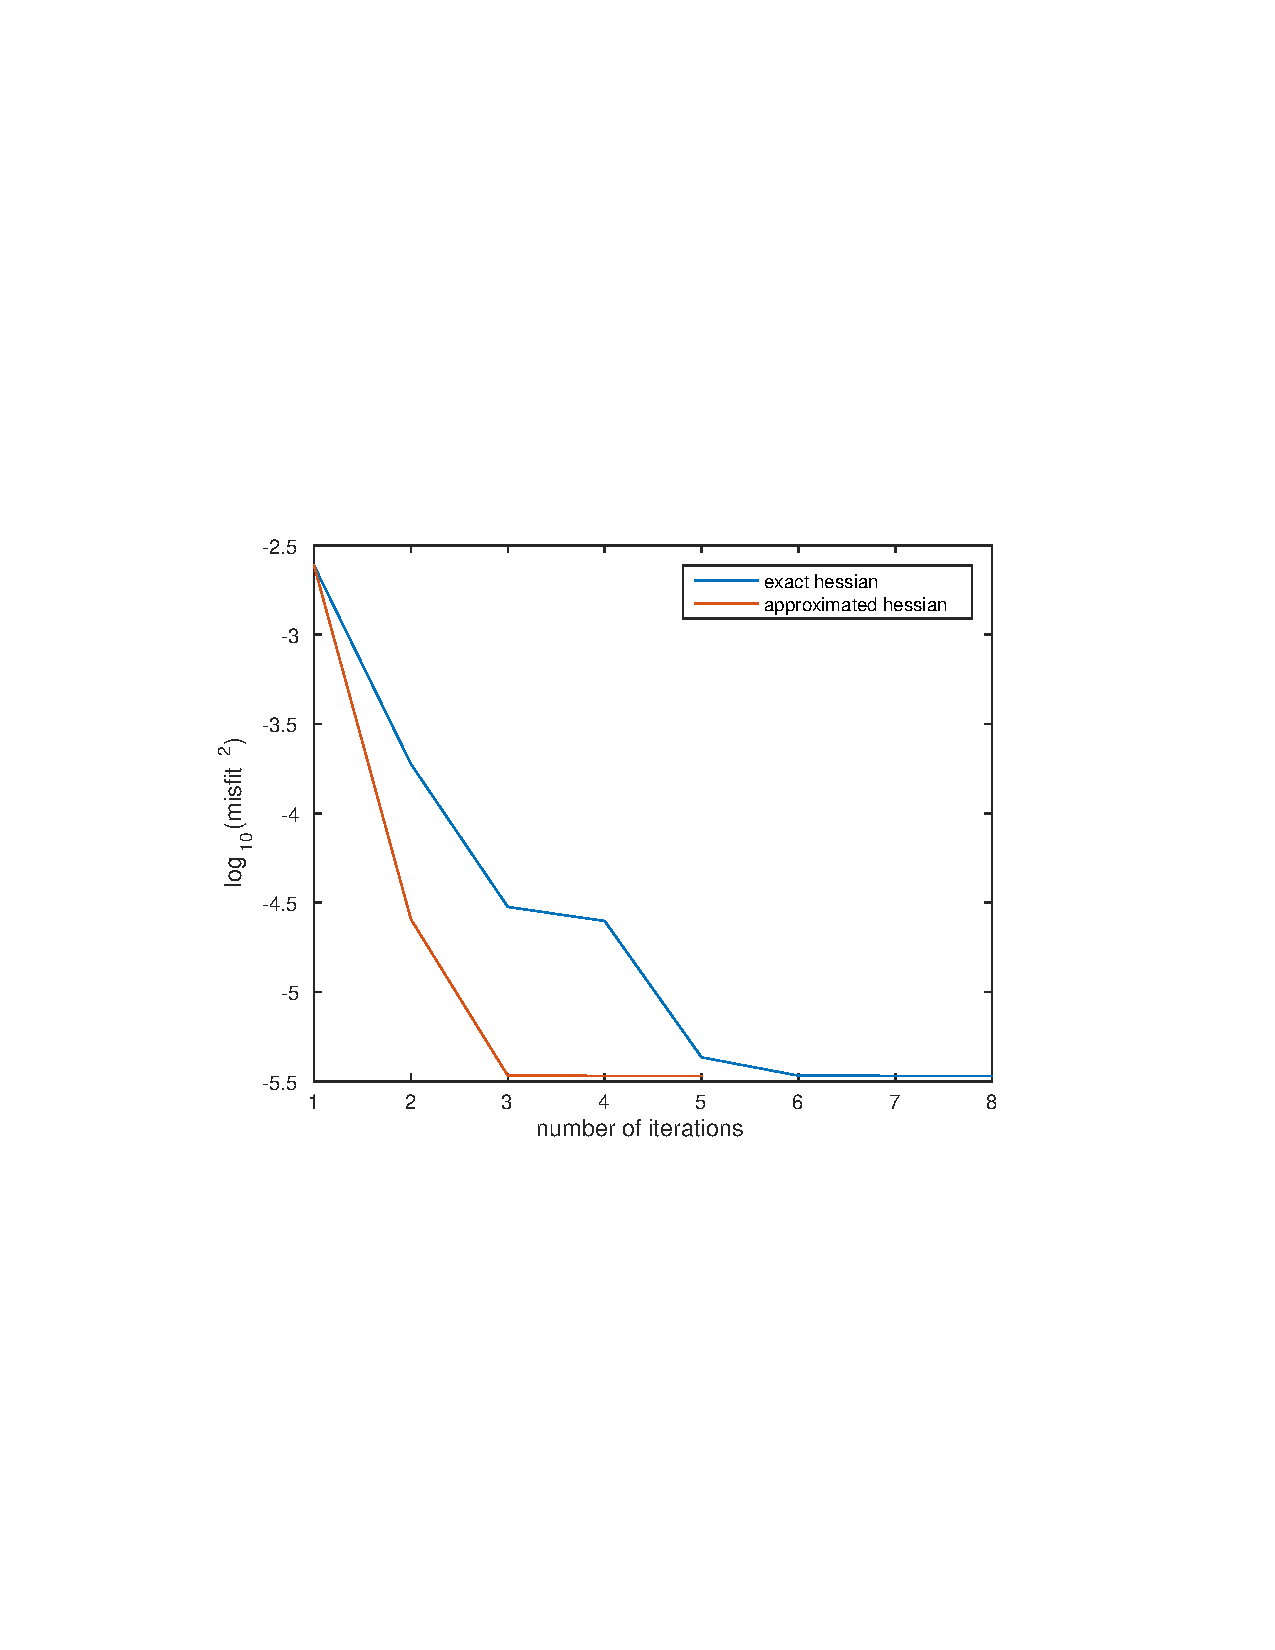
\includegraphics[bb=100bp 100bp 500bp 600bp,scale=0.8]{exact_hessian_approx_hessian_compare}

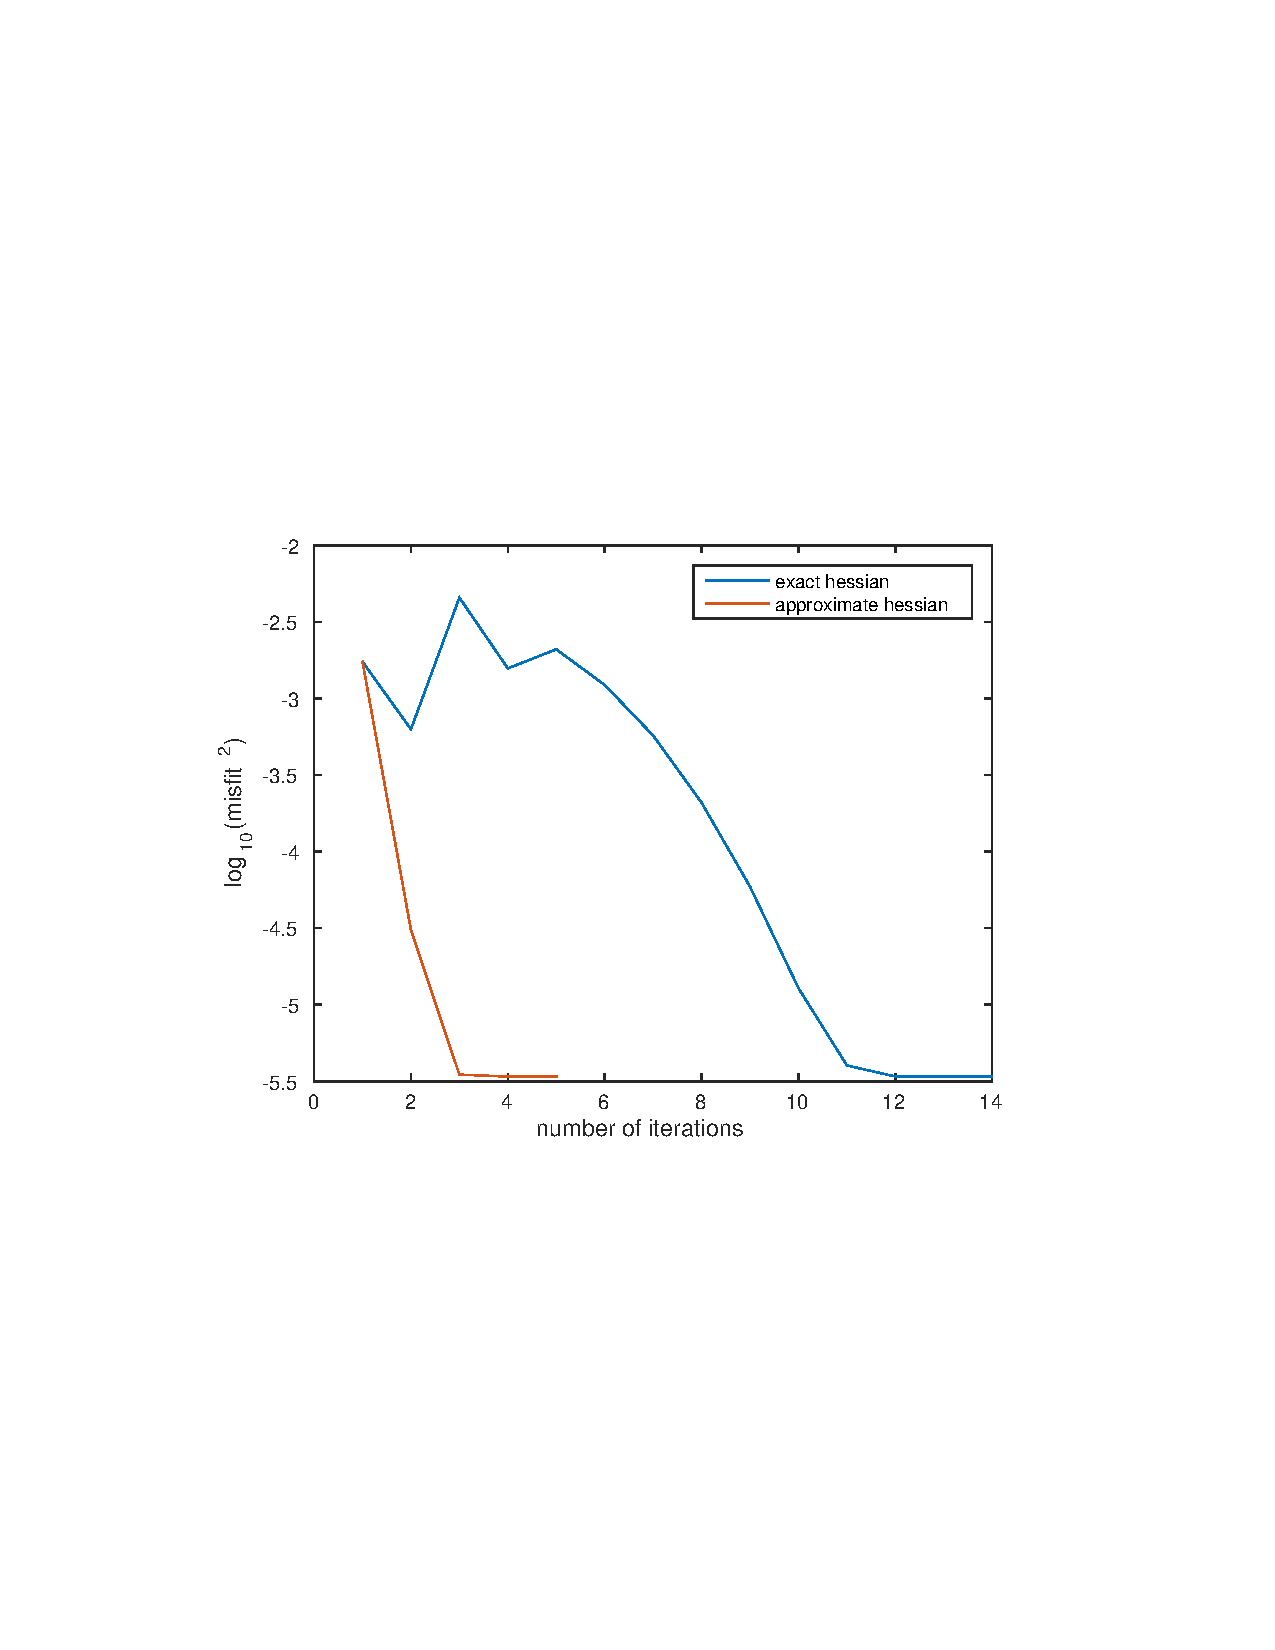
\includegraphics[bb=100bp 100bp 500bp 600bp,scale=0.8]{exact_hessian_approx_hessian_compare_1}


\subsubsection*{(b) - 10 points}


\subsubsection*{(b.i)}

Change variable $t=1/\sigma$, then 
\begin{eqnarray*}
\int_{0}^{\infty}\frac{1}{\sigma^{N}}\exp\left(-\frac{1}{2\sigma^{2}}A\right)d\sigma & = & \int_{0}^{\infty}t^{N-2}\exp\left(-\frac{A}{2}t^{2}\right)dt
\end{eqnarray*}
Since 
\begin{eqnarray*}
\int_{0}^{\infty}\exp\left(-\frac{A}{2}t^{2}\right)dt=\sqrt{\frac{\pi}{2}}A^{-1/2}\propto A^{-1/2}\\
\int_{0}^{\infty}t\exp\left(-\frac{A}{2}t^{2}\right)dt=A^{-1}\propto A^{-1}
\end{eqnarray*}
Take derivative with respect to A, then 
\begin{eqnarray*}
\int_{0}^{\infty}\frac{-t^{2}}{2}\exp\left(-\frac{A}{2}t^{2}\right)dt\propto A^{-1/2-1}\\
\int_{0}^{\infty}t\frac{-t^{2}}{2}\exp\left(-\frac{A}{2}t^{2}\right)dt\propto A^{-1-1}\\
\end{eqnarray*}
Continue this derivative, we have 
\begin{eqnarray*}
\int_{0}^{\infty}\left(\frac{-t^{2}}{2}\right)^{(N-2)/2}\exp\left(-\frac{A}{2}t^{2}\right)dt\propto A^{-1/2-(N-2)/2}
\end{eqnarray*}
So 
\begin{eqnarray*}
\int_{0}^{\infty}t^{N-2}\exp\left(-\frac{A}{2}t^{2}\right)dt\propto A^{-(N-1)/2}
\end{eqnarray*}



\subsubsection*{(b.ii)}

Assume uniform prior, then 
\begin{eqnarray*}
P(x,y|d) & \propto & P(d|x,y)=\exp-F(x,y)\\
 & = & \exp\left(-F(x_{0},y_{0})-gradF|_{x_{0},y_{0}}\cdot(x-x_{0},y-y_{0})'-\frac{1}{2}(x-x_{0},y-y_{0})H|_{x_{0},y_{0}}(x-x_{0},y-y_{0})'\right)
\end{eqnarray*}


Since at $(x_{0},y_{0})$, $gradF=0$, thus 
\begin{eqnarray*}
P(x,y|d) & \propto & \exp\left(-\frac{1}{2}(x-x_{0},y-y_{0})H|_{x_{0},y_{0}}(x-x_{0},y-y_{0})'\right)
\end{eqnarray*}


write $H$ as 
\begin{eqnarray*}
H=\begin{pmatrix}A & B\\
B & C
\end{pmatrix}
\end{eqnarray*}
thus the joint pdf will be

\begin{eqnarray*}
f(x,y)=K\exp\left(-\frac{1}{2}[A(x-x_{0})^{2}+2B(x-x_{0})(y-y_{0})+C(y-y_{0})^{2}]\right)
\end{eqnarray*}
where $K$ is the constant that normalize the pdf, to get it, we have

\begin{eqnarray*}
\int_{-\infty}^{\infty}dy\int_{-\infty}^{\infty}dxf(x,y) & = & \int_{-\infty}^{\infty}dy\int_{-\infty}^{\infty}dxK\exp\left(-\frac{1}{2}[A(x-x_{0})^{2}+2B(x-x_{0})(y-y_{0})+C(y-y_{0})^{2}]\right)\\
 & = & \int_{-\infty}^{\infty}dy\int_{-\infty}^{\infty}dxK\exp\left(-\frac{1}{2}[Ax^{2}+2Bxy+Cy^{2}]\right)\\
 & = & \int_{-\infty}^{\infty}dy\int_{-\infty}^{\infty}dxK\exp\left(-\frac{1}{2}[A(x+By/A)^{2}+(C-B^{2}/A)y^{2}]\right)\\
 & = & \int_{-\infty}^{\infty}dyK\exp\left(-\frac{1}{2}(C-B^{2}/A)y^{2}\right)\int_{-\infty}^{\infty}dx\exp\left(-\frac{1}{2}[A(x+By/A)^{2}]\right)\\
 & = & \int_{-\infty}^{\infty}dyK\exp\left(-\frac{1}{2}(C-B^{2}/A)y^{2}\right)\int_{-\infty}^{\infty}dx\exp\left(-\frac{1}{2}Ax^{2}\right)\\
 & = & \int_{-\infty}^{\infty}dyK\exp\left(-\frac{1}{2}(C-B^{2}/A)y^{2}\right)\sqrt{2\pi/A}\\
 & = & K\sqrt{2\pi/(C-B^{2}/A)}\sqrt{2\pi/A}\\
 & = & 2\pi K/\sqrt{AC-B^{2}}\\
 & = & 1
\end{eqnarray*}


Now we want to show $E[x]=x_{0}$. This is true because 
\begin{eqnarray*}
E[x-x_{0}] & = & \int_{-\infty}^{\infty}dy\int_{-\infty}^{\infty}dx\quad(x-x_{0})f(x,y)\\
 & \propto & \int_{-\infty}^{\infty}dy\int_{-\infty}^{\infty}dx\quad(x-x_{0})\exp\left(-\frac{1}{2}[A(x-x_{0})^{2}+2B(x-x_{0})(y-y_{0})+C(y-y_{0})^{2}]\right)\\
 & \propto & \int_{-\infty}^{\infty}dy\int_{-\infty}^{\infty}dx\quad x\exp\left(-\frac{1}{2}[Ax^{2}+2Bx(y-y_{0})+C(y-y_{0})^{2}]\right)\\
 & \propto & \int_{-\infty}^{\infty}dy\int_{-\infty}^{\infty}dx\quad x\exp\left(-\frac{1}{2}[Ax^{2}+2Bxy+Cy^{2}]\right)\\
 & \propto & \int_{-\infty}^{\infty}dy\int_{-\infty}^{\infty}dx\quad x\exp\left(-\frac{1}{2}[A(x+By/A)+(C-B^{2}/A)y^{2}]\right)\\
 & \propto & \int_{-\infty}^{\infty}dy(By/A)\exp\left(-\frac{1}{2}[(C-B^{2}/A)y^{2}]\right)\\
 & \propto & \int_{-\infty}^{\infty}dy\quad y\exp\left(-\frac{1}{2}[(C-B^{2}/A)y^{2}]\right)\\
 & = & 0
\end{eqnarray*}
So similarly $E[y]=y_{0}$.

Thus 
\begin{eqnarray*}
\sigma_{x}^{2} & = & E[(x-E[x])^{2}]\\
 & = & E[(x-x_{0})^{2}]\\
 & = & \int_{-\infty}^{\infty}dy\int_{-\infty}^{\infty}dx\quad\frac{\partial f(x,y)}{\partial A}/(-1/2)\\
 & = & -2\frac{\partial}{\partial A}\int_{-\infty}^{\infty}dy\int_{-\infty}^{\infty}dx\quad f(x,y)\\
 & = & -2\frac{\partial}{\partial A}2\pi K/\sqrt{AC-B^{2}}\\
 & = & \frac{2\pi K}{(A-B^{2}/C)\sqrt{AC-B^{2}}}\\
 & = & \frac{C}{AC-B^{2}}
\end{eqnarray*}
Similarly 
\begin{eqnarray*}
\sigma_{y}^{2} & = & \frac{A}{AC-B^{2}}
\end{eqnarray*}


\begin{eqnarray*}
\sigma_{xy} & = & E[(x-E[x])(y-E[y])]\\
 & = & E[(x-x_{0})(y-y_{0})]\\
 & = & \int_{-\infty}^{\infty}dy\int_{-\infty}^{\infty}dx\quad\frac{\partial f(x,y)}{\partial B}/(-1)\\
 & = & -\frac{\partial}{\partial B}\int_{-\infty}^{\infty}dy\int_{-\infty}^{\infty}dx\quad f(x,y)\\
 & = & \frac{-B}{AC-B^{2}}
\end{eqnarray*}


Note that 
\begin{eqnarray*}
\begin{pmatrix}A & B\\
B & C
\end{pmatrix}^{-1}=\frac{1}{AC-B^{2}}\begin{pmatrix}C & -B\\
-B & A
\end{pmatrix}
\end{eqnarray*}
Thus we get what we want.


\subsection*{Problem 2 (graded by Dunzhu \& Toby) 20 points}


\subsubsection*{(b) (10 points)}

Here are some topics people mentioned about the ABT book: 
\begin{itemize}
\item Appendix A, background knowledge 
\item Number of data points vs number of model parameter, overdetermined,
underdeterminined, mixed determinied 
\item MAP and Bayes' theorem 
\item L1 norm is better when existence of outlier 
\item difficulty in inverse: existance, uniqueness, and instability 
\item Fredholm integration equation of the first kind generalize many inverse
problem 
\item Chapter 11 Section 3, general multivarate normal case with prior 
\item damped Newton's method, choose the step length instead of using full
newton step 
\item ABT mentioned p-values, chi-square statistics 
\item in lecture, we maximize $P(d|m)$ to get the maximum likelihood, in
ABT they defined $L(m|d)=P(d|m)$ first, then maximize it. ABT one
is more clear, because $P(d|m)$ apprears to be a function of $d$,
where in fact we want it to be a function of $m$. 
\end{itemize}

\subsubsection*{(c) (10 points)}

Here are some topics people mentioned: 
\begin{itemize}
\item When estimating $\sigma^{2}$, devided by $N-1$ instead of $N$ 
\item Confused about $J(m)$ and $G(m)$, it's really the same thing, Jacobian 
\item class did a better job of describing prior 
\item Class and ABT does not cover the case when prior is a given range 
\item numerical calculation of derivative when it's hard to do it analytically 
\item any method for finding global minimum? \end{itemize}

\end{document}
